\documentclass[../main.tex]{subfiles}
\graphicspath{{\subfix{../figures/}}}
%
\begin{document}
\section{门面模式(Facade)}
\textbf{门面模式}:外部与子系统的通信必需通过一个统一的门面(facade)对象进行.
门面模式是对象形式的结构型设计模式.
门面模式提供一个高层次的接口,使得子系统更易于使用.

\textbf{基于模块化的子系统划分}:
\begin{itemize}
  \item 大型的软件系统都是比较复杂的,软件设计的重要任务之一就是要合理控制软件复杂性.
  \item 处理复杂系统的一个常见方法便是将其``分而治之'',把一个系统划分为几个较小的子系统.
  \item 而使用一个子系统的客户端往往需要同时与子系统内部的许多对象交互.
\end{itemize}
%
\textbf{什么情况下使用门面模式}:
\begin{itemize}
  \item \textbf{为一个复杂子系统提供一个简单接口}:子系统往往因为不断演化而变得越来越复杂,使用门面模式可以使得子系统更具有可复用性.Facade模式可以提供一个简单的操作视图.
  \item \textbf{提高子系统的独立性}:一般而言,子系统和其他的子系统之间、客户端与实现层之间存在着很大的依赖性.引入Facade模式将一个子系统与它的客户端以及其他的子系统分离,可以提高子系统的独立性和可移植性.
  \item \textbf{形成层次化结构}:在构建一个层次化的系统时,可以使用Facade模式定义系统中每一层的入口.如果层与层之间是相互依赖的,则可以限定它们仅通过Facade进行通信,从而简化了层与层之间的依赖关系.
\end{itemize}
%
\textbf{迪米特法则}:
迪米特法则说:``只与你直接的朋友们通信''.迪米特法要求每一个对象与其他对象的相互作用均是短程的,而不是长程的.只要有可能,朋友的数目越少越好.即一个对象只应当知道它的直接合作者的接口.
门面模式创造出一个门面对象,将客户端所涉及的属于一个子系统的协作伙伴的数目减到最少,使得客户端与子系统内部的对象的相互作用被门面对象所取代.

\textbf{不同子系统间对象交互}如图:
该图描述的是一个客户端必须与许多对象打交道才能完成一个功能,图中的大方框代表一个子系统.
\begin{figure}[H]
  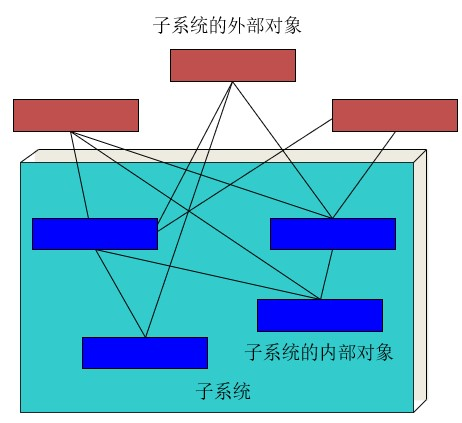
\includegraphics[width=0.35\textwidth]{25_1.jpg}
\end{figure}
%
\subsection{例子:医院}
若把医院作为一个子系统,按照部门职能,这个系统可以划分为挂号、门诊、划价、化验、收费、取药等部门.看病的病人要与这些部门打交道,就如同一个子系统的客户端与一子系统的各个类打交道一样,不是一件容易的事情.
首先病人必须挂号,然后门诊.如果医生要求化验,病人必须先 划价,然后缴款,才能到化验部门做化验.化验后,再回到门诊室.
%
\begin{figure}[H]
  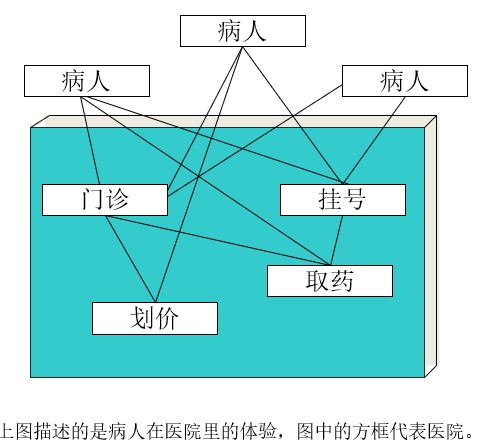
\includegraphics[width=0.45\textwidth]{25_2.jpg}
\end{figure}
%
解决这种不便的方法就是引进门面模式.
仍然通过医院的例子说明,可以设置一个导诊员的位置,由接待员负责代为挂号、划价、缴费、取药等.这个接待员就是门面模式的体现,病人只接触接待员,由接待员负责与医院的各个部门打交道,如图所示.
%
\begin{figure}[H]
  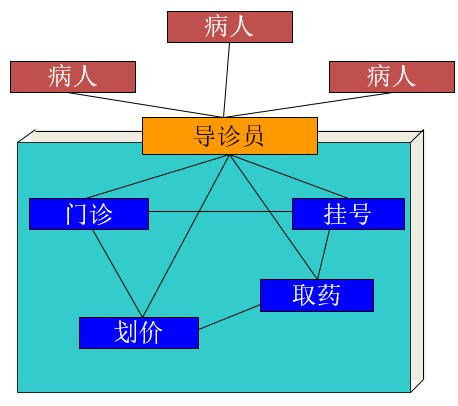
\includegraphics[width=0.45\textwidth]{25_3.jpg}
\end{figure}
%
\subsection{例子:安全监控系统}
一个安全监控系统由两个录像机、三个电灯、一个传感器和一个警报器组成.安全监控系统的操作人员需要经常将这些仪器启动和关闭.首先,在不使用门面模式的情况下,操作这个系统的操作员必须直接操作所有的这些设备.
%
\subsubsection{不使用门面模式的设计}
不使用门面模式的情况下,系统的设计图如图所示, 可看出,Client对象需要引用到所有的录象机(Camera)、电灯(Light)、感应器(Sensor)和警报器(Alarm)对象.Client对象必须对安全监控系统全知全能,这是一个高耦合度的做法.
%
\begin{figure}[H]
  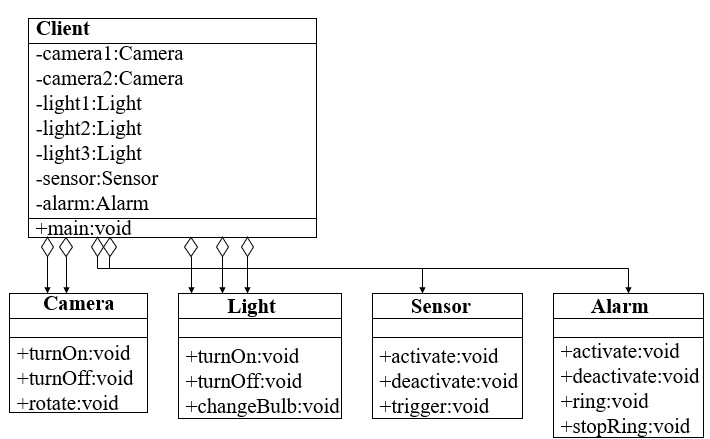
\includegraphics[width=0.65\textwidth]{25_4.jpg}
\end{figure}
%
\lstinputlisting[language=java]{./code/25/1/Camera.java}
\lstinputlisting[language=java]{./code/25/1/Light.java}
\lstinputlisting[language=java]{./code/25/1/Sensor.java}
\lstinputlisting[language=java]{./code/25/1/Alarm.java}
\lstinputlisting[language=java]{./code/25/1/Client.java}
%
\subsubsection{使用门面模式的设计}
一个合理的改进方案就是准备一个系统的控制台,作为安全监控系统的用户界面.用户只需要操作这个简化的界面就可以操控所有的内部设备,这实际上就是门面模式的用意.
使用门面模式对前面的设计方案进行改造后,就得到了如下页图所示的设计图,可以看出,门面SecurityFacade对象承担了与安全监控系统内部各个对象打交道的任务,而客户对象只需要与门面对象打交道即可.这是客户端与安全监控系统之间的一个门户,它使二者之间的关系变得简单和易于管理.
%
\begin{figure}[H]
  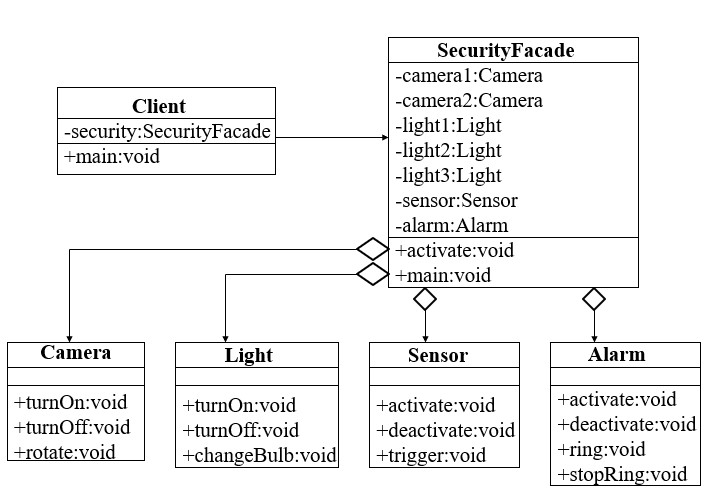
\includegraphics[width=0.65\textwidth]{25_5.jpg}
\end{figure}
%
\lstinputlisting[language=java]{./code/25/2/SecurityFacade.java}
\lstinputlisting[language=java]{./code/25/2/Client.java}
%
可以看出,客户端程序大大简化了,Client类只有一个对SecurityFacade类的引用.
\end{document}
